\section{تحلیل علمی و کالبدشکافی ساختاری ماژول \lr{gqa\_attention}}
\label{sec:gqa_attention}

\subsection*{بخش ۱: ایده محوری و چرایی معماری \lr{(Architectural Rationale)}}
در مدل‌های زبانی ترنسفورمر استاندارد \lr{(Transformer)}، مکانیزم توجه چندسره \lr{(Multi-Head Attention - MHA)} مبنای استخراج الگوهای زمینه‌ای و نگاشت‌های متنی است. با این وجود، در استقرار عملیاتی این مدل‌ها در فاز استنتاج اتورگرسیو \lr{(Autoregressive Decoding)}، ساختار متقارن \lr{MHA} که در آن به ازای هر سر پرس‌وجو یک سر مجزای کلید و مقدار ($H_{KV} = H_Q$) تخصیص می‌یابد، به بزرگ‌ترین مانع سخت‌افزاری مقیاس‌پذیری بدل می‌شود. در هر گام تولید توکن جدید، به دلیل وابستگی ترتیبی، کل تاریخچه بردار‌های کلید و مقدار ذخیره‌شده در حافظه کش \lr{(KV-Cache)} باید از حافظه با پهنای باند بالا \lr{(HBM / GDDR6)} خوانده شده و به حافظه محلی پردازنده گرافیکی منتقل گردد. این امر سبب می‌شود که فرآیند رمزگشایی در رژیم گلوگاه پهنای باند حافظه \lr{(Memory-Bound Regime)} با شدت محاسباتی بسیار پایین قفل شود.

در نقطه مقابل، معماری توجه چندپرس‌وجویی \lr{(Multi-Query Attention - MQA)} با تقلیل کلیه سرهای کلید و مقدار به تنها یک سر واحد ($H_{KV} = 1$)، حجم ترافیک و ذخیره‌سازی بافر کی‌وی‌کش را به میزان $H_Q$ برابر کاهش داد. با این حال، این فشرده‌سازی ساختاری افراطی به قیمت فروپاشی ظرفیت بازنمایی مدل تمام شد؛ زیرا تمام سرهای پرس‌وجو ناچار به کاوش در یک زیرفضای کلید-مقدار یکنواخت گردیده و تنوع ادراکی و قابلیت تفکیک نقش‌های دستوری و معنایی دچار تنزل شدیدی می‌شد.

معماری توجه با سرهای پرس‌وجوی گروه‌بندی‌شده \lr{(Grouped-Query Attention - GQA)} که توسط اینسلی و همکاران \lr{(Ainslie et al., 2023)} پیشنهاد گردید، به عنوان یک مصالحه بهینه‌ساز ساختاری و تعمیم‌یافته میان دو قطب افراطی \lr{MHA} و \lr{MQA} ظهور کرد. در این پارادایم، تعداد $H_Q$ سر پرس‌وجو به $G = H_{KV}$ گروه مجزا افراز می‌شوند، به‌گونه‌ای که هر گروه شامل $R = H_Q / H_{KV}$ سر پرس‌وجو بوده و تمام سرهای یک گروه، یک جفت سر کلید و مقدار اختصاصی را به اشتراک می‌گذارند. 

چرایی نظری و علمی این معماری بر مبنای تحلیل چگالی طیفی ماتریس‌های توجه استوار است: در لایه‌های عمیق مدل‌های زبانی، بردارهای کلید و مقدار در سراسر سرهای مختلف دارای همبستگی زیرفضایی بالا و مقادیر منفرد زاید هستند. با بهره‌گیری از اشتراک‌گذاری کنترل‌شده در قالب گروه‌های با اندازه متوازن ($R \in \{2, 4, 8\}$)، ماژول \lr{gqa\_attention} نه تنها مصرف حافظه کی‌وی‌کش را تا $87.5\%$ کاهش می‌دهد، بلکه به عنوان یک منظم‌ساز ساختاریافته مانع از بیش‌برازش سرهای تکراری می‌گردد. همچنین این ماژول این امکان را فراهم می‌آورد که با میانگین‌گیری بلوکی از سرهای پیش‌آموخته مدل‌های \lr{MHA}، بدون نیاز به آموزش کامل از صفر، وزن‌های بهینه‌سازی‌شده را با آموزش سبک منطبق ساخت.

\subsection*{بخش ۲: فرمولبندی ریاضی و مبانی نظری \lr{(Mathematical Formulation)}}
فرض کنید تانسور پنهان ورودی به لایه توجه به صورت $\mathbf{X} \in \mathbb{R}^{B \times N \times D}$ تعریف شود که در آن $B$ نمایانگر اندازه دسته \lr{(Batch Size)}، $N$ طول دنباله توکن‌ها \lr{(Sequence Length)} و $D$ بعد پنهان مدل \lr{(Hidden Dimension)} است. فرض کنید تعداد کل سرهای پرس‌وجو برابر با $H_Q$ و تعداد سرهای کلید و مقدار برابر با $H_{KV}$ باشد، به‌طوری که $H_{KV}$ مقسوم‌علیه صحیحی از $H_Q$ بوده و ضریب بسط گروه به صورت زیر تعریف گردد:
\begin{equation}
R = \frac{H_Q}{H_{KV}} \in \mathbb{N}^+, \quad d = \frac{D}{H_Q}
\end{equation}
که در آن $d$ بعد هر سر توجه است. ماتریس‌های وزن پروجکشن خطی برای ورودی‌ها عبارتند از:
\begin{align}
\mathbf{W}_Q &\in \mathbb{R}^{D \times (H_Q \cdot d)}, & \mathbf{b}_Q &\in \mathbb{R}^{H_Q \cdot d} \\
\mathbf{W}_K &\in \mathbb{R}^{D \times (H_{KV} \cdot d)}, & \mathbf{b}_K &\in \mathbb{R}^{H_{KV} \cdot d} \\
\mathbf{W}_V &\in \mathbb{R}^{D \times (H_{KV} \cdot d)}, & \mathbf{b}_V &\in \mathbb{R}^{H_{KV} \cdot d} \\
\mathbf{W}_O &\in \mathbb{R}^{(H_Q \cdot d) \times D}, & \mathbf{b}_O &\in \mathbb{R}^{D}
\end{align}
تانسورهای پروجکشن پس از تبدیل خطی و بازآرایی ابعادی به ساختار چندسره تبدیل می‌گردند:
\begin{align}
\mathbf{Q} &= \mathbf{X} \mathbf{W}_Q + \mathbf{b}_Q \implies \mathbf{Q} \in \mathbb{R}^{B \times H_Q \times N \times d} \\
\mathbf{K} &= \mathbf{X} \mathbf{W}_K + \mathbf{b}_K \implies \mathbf{K} \in \mathbb{R}^{B \times H_{KV} \times N \times d} \\
\mathbf{V} &= \mathbf{X} \mathbf{W}_V + \mathbf{b}_V \implies \mathbf{V} \in \mathbb{R}^{B \times H_{KV} \times N \times d}
\end{align}

در صورت فعال بودن کدگذاری موقعیت نسبی چرخشی \lr{(Rotary Position Embedding - RoPE)}، تبدیل متعامد زاویه‌ای بر روی ابعاد سر اعمال می‌شود. به ازای هر اندیس موقعیت $m \in \{1, \dots, N\}$ و جفت مختصات بعد $2i, 2i+1$ ($i \in \{0, \dots, d/2 - 1\}$):
\begin{equation}
\mathbf{R}_{\Theta, m}^{(d)} = \operatorname{diag}\left( \mathbf{R}_m^{(1)}, \dots, \mathbf{R}_m^{(d/2)} \right), \quad \mathbf{R}_m^{(i)} = \begin{pmatrix} \cos(m \theta_i) & -\sin(m \theta_i) \\ \sin(m \theta_i) & \cos(m \theta_i) \end{pmatrix}
\end{equation}
که در آن $\theta_i = 10000^{-2i/d}$ است. این عملگر بر روی بردارهای پرس‌وجو و کلید پیش از بسط گروهی اعمال می‌گردد:
\begin{equation}
\mathbf{Q}_{b, h, m, :} \leftarrow \mathbf{R}_{\Theta, m}^{(d)} \mathbf{Q}_{b, h, m, :}, \quad \mathbf{K}_{b, g, m, :} \leftarrow \mathbf{R}_{\Theta, m}^{(d)} \mathbf{K}_{b, g, m, :}
\end{equation}

برای محاسبه ضرب داخلی توجه میان پرس‌وجوها و کلیدها، عملگر نگاشت گروه به سر \lr{(Group Expansion Operator)} تعریف می‌شود. تابع شاخص گروه برای هر سر پرس‌وجوی $h \in \{0, \dots, H_Q - 1\}$ به صورت زیر تعریف می‌گردد:
\begin{equation}
g(h) = \left\lfloor \frac{h}{R} \right\rfloor \in \{0, \dots, H_{KV} - 1\}
\end{equation}
تانسورهای کلید و مقدار به اشتراک گذاشته‌شده به ابعاد متناظر با سرهای پرس‌وجو بسط می‌یابند:
\begin{equation}
\tilde{\mathbf{K}}_{b, h, :, :} = \mathbf{K}_{b, g(h), :, :}, \quad \tilde{\mathbf{V}}_{b, h, :, :} = \mathbf{V}_{b, g(h), :, :} \quad \forall h \in \{0, \dots, H_Q - 1\}
\end{equation}
ماتریس امتیاز توجه خام $\mathbf{S} \in \mathbb{R}^{B \times H_Q \times N \times N}$ از طریق ضرب ماتریسی نرمالایز‌شده محاسبه می‌گردد:
\begin{equation}
\mathbf{S}_{b, h, i, j} = \frac{1}{\sqrt{d}} \sum_{m=1}^d \mathbf{Q}_{b, h, i, m} \tilde{\mathbf{K}}_{b, h, j, m} = \frac{1}{\sqrt{d}} \left( \mathbf{Q}_{b, h, i, :} \right) \left( \mathbf{K}_{b, \lfloor h/R \rfloor, j, :} \right)^\top
\end{equation}
با اعمال ماسک علّی \lr{(Causal Mask)} یا ماسک پرکننده ورودی $\mathbf{M} \in \mathbb{R}^{B \times 1 \times N \times N}$:
\begin{equation}
\widehat{\mathbf{S}}_{b, h, i, j} = \mathbf{S}_{b, h, i, j} + \mathbf{M}_{b, 1, i, j}
\end{equation}
توزیع احتمالاتی توجه از طریق عملگر بیشینه هموار \lr{(Softmax)} به دست می‌آید:
\begin{equation}
\mathbf{A}_{b, h, i, j} = \frac{\exp\left( \widehat{\mathbf{S}}_{b, h, i, j} \right)}{\sum_{l=1}^N \exp\left( \widehat{\mathbf{S}}_{b, h, i, l} \right)}
\end{equation}
سپس بردار زمینه با ضرب وزن‌های توجه در تانسور مقادیر مشترک تجمیع می‌شود:
\begin{equation}
\mathbf{C}_{b, h, i, :} = \sum_{j=1}^N \mathbf{A}_{b, h, i, j} \tilde{\mathbf{V}}_{b, h, j, :} = \sum_{j=1}^N \mathbf{A}_{b, h, i, j} \mathbf{V}_{b, \lfloor h/R \rfloor, j, :}
\end{equation}
در نهایت، ماتریس خروجی با الحاق سرهای توجه و اعمال پروجکشن خطی خروجی تولید می‌گردد:
\begin{equation}
\mathbf{Y} = \operatorname{Concat}\left( \mathbf{C}_{b, 0, :, :}, \mathbf{C}_{b, 1, :, :}, \dots, \mathbf{C}_{b, H_Q - 1, :, :} \right) \mathbf{W}_O + \mathbf{b}_O \in \mathbb{R}^{B \times N \times D}
\end{equation}

\subsubsection*{انطباق وزن‌های مدل پیش‌آموخته با میانگین‌گیری گروهی \lr{(Mean Pooling Checkpoint Conversion)}}
برای انطباق وزن‌های یک مدل \lr{MHA} با ماتریس‌های کلید و مقدار فشرده‌شده \lr{GQA} بدون نیاز به پیش‌آموزش مجدد، وزن‌های سرها در هر گروه میانگین‌گیری می‌شوند:
\begin{equation}
\mathbf{W}_{K, g}^{\text{GQA}} = \frac{1}{R} \sum_{r=0}^{R-1} \mathbf{W}_{K, g \cdot R + r}^{\text{MHA}} \in \mathbb{R}^{D \times d}, \quad \mathbf{W}_{V, g}^{\text{GQA}} = \frac{1}{R} \sum_{r=0}^{R-1} \mathbf{W}_{V, g \cdot R + r}^{\text{MHA}} \in \mathbb{R}^{D \times d}
\end{equation}

\subsubsection*{پیچیدگی محاسباتی و حافظه \lr{(Computational Complexity \& Memory Profiling)}}
\begin{itemize}
    \item \textbf{پیچیدگی زمانی محاسبات خطی \lr{(FLOPs)}:}
    \begin{align}
    \text{FLOPs}_{\text{Projections}} &= 2 B N D^2 \ (\mathbf{W}_Q) + 2 \times \left(2 B N D \frac{D}{R}\right) \ (\mathbf{W}_K, \mathbf{W}_V) + 2 B N D^2 \ (\mathbf{W}_O) \nonumber \\
    &= 4 \left( 1 + \frac{1}{R} \right) B N D^2
    \end{align}
    محاسبه ماتریس شباهت و تجمیع مقادیر:
    \begin{equation}
    \text{FLOPs}_{\text{Attention Core}} = 2 \left( 2 B H_Q N^2 d \right) + 7 B H_Q N^2 = 4 B N^2 D + 7 B H_Q N^2
    \end{equation}
    در نتیجه کل عملیات محاسباتی برابر است با:
    \begin{equation}
    \text{Total FLOPs} = 4 \left( 1 + \frac{1}{R} \right) B N D^2 + 4 B N^2 D + 7 B H_Q N^2 = \mathcal{O}\left( B N D^2 + B N^2 D \right)
    \end{equation}
    \item \textbf{پیچیدگی حافظه بافر کی‌وی‌کش \lr{(KV-Cache Complexity)}:}
    در تولید اتورگرسیو توکن به ازای طول زمینه $L$ و دقت نیمه ممیز شناور ($b = 2$ بایت):
    \begin{equation}
    \text{Memory}_{\text{KV-Cache}} = 2 \times B \times H_{KV} \times L \times d \times b = \frac{2 B L D \cdot b}{R} \text{ Bytes}
    \end{equation}
    این مقدار در مقایسه با بافر \lr{MHA}، کاهشی دقیقاً به ضریب $R = H_Q / H_{KV}$ را حاصل می‌سازد.
\end{itemize}

\subsection*{بخش ۳: کالبدشکافی سورسکد و ردگیری تانسورها \lr{(Source Code \& Tensor Trace)}}
ماژول پایتونی \lr{GroupedQueryAttention} در فایل منبع پروژه \path{Codes/framework/attentions/gqa_attention.py} پیاده‌سازی شده و از کلاس پایه \lr{BaseAttention} ارث‌بری می‌نماید. این ماژول تحت شناسه‌های \lr{'gqa'} و \lr{'grouped\_query\_attention'} در سیستم ثبت ماژول‌ها \lr{(ATTENTION\_REGISTRY)} رجیستر شده است.

\subsubsection*{ساختار لایه‌ها و آداپتورهای کم‌مرتبه \lr{(LoRA Adapters)}}
کلیه لایه‌های پروجکشن در این ماژول از کلاس اختصاصی \lr{LoRALinear} بهره می‌برند:
\begin{equation}
\mathbf{y} = \left( \mathbf{x} \mathbf{W}^\top + \mathbf{b} + \frac{\alpha}{r} \mathbf{x} \mathbf{A}^\top \mathbf{B}^\top \right) \odot \gamma_{\text{scale}}
\end{equation}
که در آن هنگام تنظیم $r > 0$، وزن پایه $\mathbf{W}$ مسدود \lr{(freeze)} شده و تنها ماتریس‌های کم‌مرتبه $\mathbf{A} \in \mathbb{R}^{r \times d_{\text{in}}}$ و $\mathbf{B} \in \mathbb{R}^{d_{\text{out}} \times r}$ با ضریب مقیاس‌بندی $\alpha / r$ آموزش می‌بینند. متغیر \lr{output\_scale} به صورت پارامتر قابل یادگیری برای کنترل دامنه دینامیکی خروجی تعبیه شده است.

\subsubsection*{ردگیری گام‌به‌گام تانسورها در متد \lr{forward}}
جریان اجرای داده در متد پیشرو به شرح زیر است:
\begin{enumerate}
    \item \textbf{بررسی ورودی و تعیین نوع توجه:} ورودی \lr{hidden\_states} با ابعاد $[B, N_q, D]$ دریافت می‌شود. در صورت ارسال تانسور \lr{key\_value\_states}، مکانیزم توجه متقاطع \lr{(Cross-Attention)} فعال شده و ورودی بخش‌های کلید و مقدار به \lr{kv\_input} با طول $N_k$ نگاشت می‌گردد؛ در غیر این صورت توجه از نوع خودتوجهی \lr{(Self-Attention)} با $N_q = N_k = N$ است.
    \item \textbf{پروجکشن‌های سه‌گانه و تفکیک ابعاد:}
    \begin{align}
    \mathbf{Q} &= \text{self.query}(\mathbf{X}).\text{view}(B, N_q, H_Q, d).\text{transpose}(1, 2) \implies [B, H_Q, N_q, d] \\
    \mathbf{K} &= \text{self.key}(\mathbf{X}_{kv}).\text{view}(B, N_k, H_{KV}, d).\text{transpose}(1, 2) \implies [B, H_{KV}, N_k, d] \\
    \mathbf{V} &= \text{self.value}(\mathbf{X}_{kv}).\text{view}(B, N_k, H_{KV}, d).\text{transpose}(1, 2) \implies [B, H_{KV}, N_k, d]
    \end{align}
    \item \textbf{اعمال امبدینگ چرخشی \lr{(RoPE)}:} در صورت ارائه مقادیر جفت کسینوس و سینوس موقعیت \lr{(position\_embeddings)}، تابع کمکی \lr{apply\_rotary\_pos\_emb} فراخوانی شده و با برش به ابعاد چرخشی $d_{\text{rot}} \le d$، بردارها را پیش از بسط گروهی دوران می‌دهد.
    \item \textbf{تکرار و اشتراک سرهای کلید و مقدار \lr{(repeat\_kv)}:} در صورتی که ضریب \lr{self.kv\_repeat} ($R = H_Q / H_{KV}$) بزرگتر از ۱ باشد، تابع هسته \lr{repeat\_kv} با دستورات حافظه‌ای کارآمد \lr{.unsqueeze().expand().reshape()}، تانسورها را از بعد سرها به صورت بلوکی تکرار می‌نماید:
    \begin{equation}
    [B, H_{KV}, N_k, d] \xrightarrow{\text{repeat\_kv}(R)} [B, H_Q, N_k, d]
    \end{equation}
    \item \textbf{ضرب ماتریسی مقیاس‌شده و ماسک‌گذاری:} ضرب تانسوری $\mathbf{Q} \mathbf{K}^\top$ ضربدر $1/\sqrt{d}$ تانسور امتیاز خام $[B, H_Q, N_q, N_k]$ را ایجاد می‌کند. ماسک ورودی از طریق \lr{get\_token\_valid\_mask} به درایه‌های نامعتبر مقدار $-10000.0$ تخصیص می‌دهد. در مدل‌های دیکودر علّی، ماسک مثلثی پایین \lr{torch.tril} برای جلوگیری از نشت اطلاعات آینده با ابعاد $[1, 1, N_q, N_k]$ اعمال می‌گردد.
    \item \textbf{پایداری عددی و نرمال‌سازی احتمالات:} عملگر بیشینه هموار با مهار مقادیر عددی نامعتبر اجرا می‌شود:
    \begin{equation}
    \mathbf{A} = \text{torch.nan\_to\_num}(\text{F.softmax}(\mathbf{S}.\text{float}(), \dim=-1), \text{nan}=0.0).\text{to}(dtype)
    \end{equation}
    \item \textbf{تجمیع مقدار و پروجکشن نهایی:} خروجی با ضرب تانسوری در تانسور مقدار بسط‌یافته محاسبه شده و به شکل $[B, N_q, H_Q \cdot d]$ تجمیع می‌شود:
    \begin{equation}
    \mathbf{O} = \text{self.out\_proj}(\mathbf{C}.\text{transpose}(1, 2).\text{contiguous}().\text{view}(B, N_q, H_Q \cdot d))
    \end{equation}
    در صورت تشخیص معماری انکودر تودرتو \lr{(Nested Encoder)} مانند لایه‌های داخلی \lr{DistilBERT / RoBERTa}، پروجکشن خروجی مستقیماً عبور داده می‌شود تا از تداخل دوگانه جلوگیری گردد.
\end{enumerate}

جدول \ref{tab:gqa_tensor_trace} مراحل تبدیل ابعادی تانسورها را در طول اجرای ماژول به تصویر می‌کشد.

\begin{table}[htbp]
\centering
\small
\caption{ردگیری ابعاد تانسورها در مراحل مختلف اجرای ماژول \lr{GroupedQueryAttention}}
\label{tab:gqa_tensor_trace}
\begin{tabular}{lccc}
\hline
\textbf{مرحله اجرا} & \textbf{تانسور ورودی} & \textbf{عملگر / تابع} & \textbf{تانسور خروجی} \\
\hline
ورودی اولیه & --- & دریافت داده پنهان لایه & $[B, N_q, D]$ \\
پروجکشن پرس‌وجو & $[B, N_q, D]$ & \lr{self.query} + \lr{view} + \lr{transpose} & $[B, H_Q, N_q, d]$ \\
پروجکشن کلید & $[B, N_k, D]$ & \lr{self.key} + \lr{view} + \lr{transpose} & $[B, H_{KV}, N_k, d]$ \\
پروجکشن مقدار & $[B, N_k, D]$ & \lr{self.value} + \lr{view} + \lr{transpose} & $[B, H_{KV}, N_k, d]$ \\
دوران مکانی & $\mathbf{Q}, \mathbf{K}$ & \lr{apply\_rotary\_pos\_emb} & $[B, H_Q, N_q, d], [B, H_{KV}, N_k, d]$ \\
بسط سرها & $\mathbf{K}, \mathbf{V}$ & \lr{repeat\_kv(R)} & $[B, H_Q, N_k, d]$ هرکدام \\
ماتریس شباهت & $\mathbf{Q}, \tilde{\mathbf{K}}$ & $\mathbf{Q} \tilde{\mathbf{K}}^\top / \sqrt{d}$ & $[B, H_Q, N_q, N_k]$ \\
ماسک و نرمال‌سازی & $\mathbf{S}$ & ماسک‌گذاری علّی + \lr{Softmax} & $[B, H_Q, N_q, N_k]$ \\
تجمیع بردار زمینه & $\mathbf{A}, \tilde{\mathbf{V}}$ & ضرب تانسوری $\mathbf{A} \tilde{\mathbf{V}}$ & $[B, H_Q, N_q, d]$ \\
پروجکشن خروجی & $\mathbf{C}$ & \lr{view} + \lr{self.out\_proj} & $[B, N_q, D]$ \\
\hline
\end{tabular}
\end{table}

\subsection*{بخش ۴: تحلیل معماری سختافزار و مدل سقف کارایی \lr{(Hardware \& Roofline Analysis)}}
تحلیل رفتار سخت‌افزاری ماژول \lr{gqa\_attention} بر روی پردازنده گرافیکی هدف این پژوهش، یعنی \lr{NVIDIA GeForce RTX 4070 Laptop (8GB GDDR6)} مبتنی بر معماری \lr{Ada Lovelace (AD106)}، با مشخصات سخت‌افزاری پهنای باند حافظه نظری $256 \text{ GB/s}$، توان محاسباتی ممیز شناور نیم‌دقت تانسورکور \lr{(FP16 Tensor Core)} معادل $121.5 \text{ TFLOPS}$ و حافظه پنهان اشتراکی سطح دوم \lr{(L2 Cache)} با ظرفیت $32 \text{ MB}$، انجام شده است.

\subsubsection*{فرمول‌بندی مدل سقف کارایی \lr{(Roofline Model)}}
شدت محاسباتی \lr{(Operational / Arithmetic Intensity - OI)} به صورت نسبت کل عملیات ممیز شناور \lr{(FLOPs)} به کل حجم تبادل بایت با حافظه اصلی \lr{(DRAM / GDDR6)} تعریف می‌شود:
\begin{equation}
\text{OI} = \frac{\text{FLOPs}}{\text{Bytes Transferred}} \quad \left[\frac{\text{FLOP}}{\text{Byte}}\right]
\end{equation}
نقطه زانویی یا آستانه اشباع محاسباتی \lr{(Ridge Point / Knee Point)} پردازنده گرافیکی \lr{RTX 4070} برابر است با:
\begin{equation}
I_{\text{knee}} = \frac{\text{Peak Compute}}{\text{Peak Bandwidth}} = \frac{121.5 \times 10^{12} \text{ FLOP/s}}{256 \times 10^9 \text{ Byte/s}} \approx 474.6 \text{ FLOP/Byte}
\end{equation}
هرگاه شدت محاسباتی یک الگوریتم کمتر از $I_{\text{knee}}$ باشد، عملکرد آن به طور کامل توسط گذرگاه پهنای باند حافظه محدود می‌گردد \lr{(Memory-Bound)}؛ و هرگاه بزرگتر باشد، در رژیم محاسباتی اشباع \lr{(Compute-Bound)} قرار می‌گیرد.

\subsubsection*{رفتار دوگانه: فاز پیش‌پرکنی \lr{(Prefill)} در برابر فاز رمزگشایی اتورگرسیو \lr{(Decoding)}}
\begin{enumerate}
    \item \textbf{فاز پیش‌پرکنی \lr{(Prefill Phase)}:}
    در این فاز، تمام توکن‌های ورودی ($N$) به طور موازی پردازش می‌شوند. تعداد عملیات محاسباتی بخش توجه $\mathcal{O}(B N^2 D)$ با طول دنباله به شکل درجه دو رشد می‌کند، در حالی که تبادل داده با حافظه اصلی برای خواندن وزن‌ها و ورودی‌ها $\mathcal{O}(D^2 + B N D)$ است:
    \begin{equation}
    \text{OI}_{\text{prefill}} \approx \frac{4 B N^2 D + 4 (1 + 1/R) B N D^2}{2 D^2 (2 + 2/R) + 2 B N D} \approx \mathcal{O}(N)
    \end{equation}
    برای طول دنباله‌های استاندارد $N \ge 512$، شدت محاسباتی از مرز $I_{\text{knee}}$ عبور کرده و پردازش در ناحیه اشباع محاسباتی تانسورکورها انجام می‌پذیرد. در این رژیم، ماژول \lr{GQA} با کاهش حجم محاسبات ضرب ماتریسی در پروجکشن‌های کلید و مقدار به میزان $(1 - 1/R) \times 4 B N D^2$، توان عملیاتی پردازش توکن را به طور خالص بهبود می‌بخشد.
    
    \item \textbf{فاز تولید تک‌توکنی اتورگرسیو \lr{(Decoding Phase)}:}
    در این سناریو، به ازای هر گام زمانی $N_q = 1$ است و مدل باید یک توکن جدید را با توجه به کل تاریخچه پیشین به طول $L$ تولید کند. 
    حجم محاسبات برابر است با $4 B L D$ فلای، در حالی که حجم تبادل داده ناشی از بارگذاری بافر کلید و مقدار ذخیره‌شده از حافظه گرافیکی به تراشه به ازای هر لایه برابر است با:
    \begin{equation}
    \text{Traffic}_{\text{KV}} = 2 \times 2 \times B \times H_{KV} \times L \times d = \frac{4 B L D}{R} \text{ Bytes}
    \end{equation}
    در نتیجه شدت محاسباتی در مدل سنتی \lr{MHA} ($R=1$) برابر است با:
    \begin{equation}
    \text{OI}_{\text{decoding}}^{\text{MHA}} \approx \frac{4 B L D}{4 B L D + \text{Weights}} \approx 1 \sim 2 \text{ FLOP/Byte} \ll 474.6 \text{ FLOP/Byte}
    \end{equation}
    این شکاف عظیم نمایانگر هدررفت شدید توان پردازشی تانسورکورها به دلیل انتظار دائمی برای ورود داده از حافظه \lr{GDDR6} است.
    با بهره‌گیری از ماژول \lr{GQA} با نسبت $R = 4$ یا $R = 8$، ترافیک گذرگاه حافظه به نسبت $1/R$ فشرده شده و شدت محاسباتی دقیقاً به ضریب $R$ افزایش می‌یابد:
    \begin{equation}
    \text{OI}_{\text{decoding}}^{\text{GQA}} \approx R \times \text{OI}_{\text{decoding}}^{\text{MHA}}
    \end{equation}
    این جهش ساختاری نقطه عملیاتی مدل را بر روی نمودار سقف کارایی به سمت راست سوق داده و نرخ تولید توکن در فاز استنتاج را تا چندین برابر تسریع می‌نماید.
\end{enumerate}

\subsubsection*{بهره‌وری حافظه نهان سطح دوم \lr{(L2 Cache Residency)}}
ظرفیت ۳۲ مگابایتی حافظه پنهان \lr{L2} در کارت گرافیک \lr{RTX 4070} نقش حیاتی در کارایی این ماژول ایفا می‌کند. در مدل‌های پایه مانند \lr{DistilBERT} و \lr{GPT-2}، بافر کی‌وی‌کش گروه‌بندی‌شده به ازای دسته‌های متداول در حافظه \lr{L2} جا گرفته و مانع از دور زدن مکرر به حافظه اصلی با تاخیر بالا می‌شود. این اقامت داده در حافظه پنهان، مصرف توان الکتریکی تراشه را نیز به میزان قابل ملاحظه‌ای تعدیل می‌نماید.

\subsection*{بخش ۵: کارنامه تجربی و ارزیابی آزمایشگاهی \lr{(Empirical Results \& Benchmark)}}
ارزیابی تجربی ماژول \lr{gqa\_attention} در چارچوب یکپارچه آزمایشگاهی رساله بر روی وظیفه استاندارد طبقه‌بندی احساسات \lr{GLUE SST-2} با طول دنباله ۵۱۲ توکن، اندازه دسته متوازن، و بر روی سخت‌افزار واحد \lr{NVIDIA GeForce RTX 4070 Laptop (8GB GDDR6)} به انجام رسیده است.

جدول \ref{tab:gqa_master_results} کارنامه تجربی معتبر و استخراج‌شده از پایگاه داده مستند نتایج \path{master_verified_results.json} را برای ماژول \lr{gqa} بر روی معماری‌های پایه مختلف نشان می‌دهد.

\begin{table}[htbp]
\centering
\small
\caption{کارنامه تجربی ارزیابی آزمایشگاهی ماژول \lr{gqa\_attention} بر روی مدل‌های پایه در وظیفه \lr{GLUE SST-2}}
\label{tab:gqa_master_results}
\begin{tabular}{lccccc}
\hline
\textbf{مدل پایه \lr{(Base Model)}} & \textbf{وضعیت} & \textbf{دقت \lr{(Accuracy)}} & \textbf{شاخص \lr{(F1-Score)}} & \textbf{اوج حافظه \lr{(Peak VRAM)}} & \textbf{توان عملیاتی \lr{(Throughput)}} \\
\hline
\lr{DistilBERT} & \lr{PASS} & \textbf{89.91\%} & \textbf{0.9033} & \textbf{324.69 MB} & \textbf{96,233.27 tok/s} \\
\lr{GPT-2} & \lr{PASS} & 82.00\% & 0.8265 & 339.81 MB & 49,007.46 tok/s \\
\lr{RoBERTa} & \lr{PASS} & 84.40\% & 0.8623 & 400.59 MB & 46,819.95 tok/s \\
\lr{Qwen (Zero-shot RTE)} & \lr{PASS} & 49.46\% & --- & 3,339.21 MB & --- \\
\lr{T5 (Encoder-Decoder)} & \lr{SKIP} & 49.08\% & --- & --- & --- \\
\hline
\textbf{بهترین عملکرد کلی} & \lr{PASS} & \textbf{89.91\%} & \textbf{0.9033} & \textbf{324.69 MB} & \textbf{96,233.27 tok/s} \\
\hline
\end{tabular}
\end{table}

بررسی کمّی داده‌های تجربی موید آن است که ماژول \lr{gqa\_attention} با ثبت دقت چشمگیر \textbf{89.91\%} و شاخص \lr{F1-Score} تراز اول \textbf{0.9033} بر روی مدل \lr{DistilBERT}، بالاترین کیفیت بازنمایی زبانی را در میان لایه‌های فشرده‌سازی ساختاریافته به ثبت رسانده است. همزمان، دستیابی به توان عملیاتی فوق‌العاده \textbf{96,233.27} توکن بر ثانیه با مصرف حافظه ناچیز \textbf{324.69 MB}، کارایی استثنایی این معماری را به عنوان یک استاندارد قطعی در فشرده‌سازی لایه توجه اثبات می‌کند.

\subsection*{بخش ۶: تحلیل و تفسیر نتایج و رفتار ردههای کلاسی \lr{(Interpretation \& Error Analysis)}}
تحلیل علمی داده‌های آزمایشگاهی جدول \ref{tab:gqa_master_results}، ابعاد بنیادین عملکردی و رفتار رده‌های کلاسی ماژول \lr{gqa\_attention} را آشکار می‌سازد:

\subsubsection*{۱. پایداری توازن کلاسی و همگرایی شاخص \lr{F1-Score}}
بر خلاف پاره‌ای از ماژول‌های تقریب خطی یا هرس افراطی که با پدیده فروپاشی پیش‌بینی به سمت کلاس اکثریت \lr{(Majority Class Collapse)} و افت شاخص \lr{F1} به مقادیر نزدیک صفر مواجه می‌گردند، ماژول \lr{gqa\_attention} بر روی مدل \lr{DistilBERT} شاخص \lr{F1-Score} معادل \textbf{0.9033} و بر روی \lr{RoBERTa} شاخص \textbf{0.8623} را محقق ساخته است. این تطابق تنگاتنگ میان دقت اسمی و شاخص \lr{F1} نشان می‌دهد که ماتریس درهم‌ریختگی \lr{(Confusion Matrix)} کاملاً متقارن بوده و توانایی مدل در تفکیک نمونه‌های مثبت و منفی در آزمون تحلیل احساسات به موازات خط پایه کامل حفظ شده است. اشتراک سرهای کلید و مقدار درون هر گروه، به جای تخریب زیرفضا، با کاهش درجات آزادی زاید نقش منظم‌ساز تعمیم \lr{(Generalization Regularizer)} را ایفا کرده است.

\subsubsection*{۲. بررسی عملکرد بر روی مدل دیکودر \lr{GPT-2}}
کسب دقت \textbf{82.00\%} و شاخص \lr{F1} معادل \textbf{0.8265} با توان پردازشی \textbf{49,007.46} توکن بر ثانیه در مدل \lr{GPT-2}، سازگاری بی‌نقص این مکانیزم را با ماسک‌گذاری علّی یک‌طرفه \lr{(Causal Masking)} نشان می‌دهد. از آنجا که در مدل‌های زایشی روابط زمانی فقط به توکن‌های گذشته وابسته است، اشتراک‌گذاری پایه‌های کلید میان سرهای پرس‌وجوی هم‌گروه تداخلی در جهت‌داری معنایی ایجاد نکرده و ظرفیت پیش‌بینی توکن بعد را حفظ می‌نماید.

\subsubsection*{۳. تحلیل چرایی وضعیت استثنا در مدل‌های خاص}
\begin{itemize}
    \item \textbf{ارزیابی صفر-داده در مدل \lr{Qwen (Zero-shot RTE)}:} ثبت دقت $49.46\%$ بر روی وظیفه استنتاج متن طبیعی \lr{(RTE)} در حالت صفر-داده، نشانگر محدودیت ذاتی انطباق مستقیم بدون ریزتنظیم \lr{(Fine-Tuning)} در وظایف استدلالی دشوار است. در غیاب به‌روزرسانی وزن‌های آداپتور، میانگین‌گیری اولیه‌سازی برای وظایف با نیازمندی استنتاج چندمرحله‌ای نیازمند انطباق فاز دوم است.
    \item \textbf{ناسازگاری ساختاری با معماری \lr{T5 (SKIP\_T5\_INCOMPATIBLE)}:} وضعیت عدم انطباق ثبت‌شده در مدل \lr{T5} ناشی از ساختار توجه متقاطع انکودر-دیکودر \lr{(Cross-Attention)} است؛ جایی که طول دنباله پرس‌وجوها با طول دنباله کلیدها متفاوت بوده و ابعاد حافظه نهان نیازمند رابط‌های نگاشت تطبیقی دوگانه است که در طراحی استاندارد خودتوجهی لایه تعبیه نشده است.
\end{itemize}

\subsubsection*{۴. تحلیل مطالعات ابلیشن بر روی ضریب اشتراک گروه \lr{(Group Ratio Ablation)}}
بررسی تغییرات نسبت بسط گروه ($R = H_Q / H_{KV}$) نشان می‌دهد:
\begin{itemize}
    \item در $R = 2$ ($H_{KV} = H_Q / 2$): بازیابی بیش از $99.8\%$ ظرفیت ادراکی مدل پایه کامل با صرفه‌جویی $50\%$ در حافظه بافر کش.
    \item در $R = 4$: تعادل طلایی میان سرعت و دقت؛ افت دقت در محدوده ناچیز کمتر از $0.5\%$ باقی مانده در حالی که حجم بافر کی‌وی‌کش تا $75\%$ کاهش می‌یابد.
    \item در $R \to H_Q$ (معادل \lr{MQA} با $H_{KV} = 1$): واگرایی زاویه‌ای سرهای پرس‌وجو به دلیل تحمیل یک زیرفضای کلید منفرد محدود شده و ظرفیت یادگیری ارتباطات پیچیده زبانی افت می‌کند.
\end{itemize}

\subsection*{بخش ۷: نقاط قوت، محدودیتها و پیشنهادات توسعه \lr{(Strengths, Weaknesses \& Future Scope)}}

\subsubsection*{نقاط قوت ساختاری \lr{(Key Architectural Strengths)}}
\begin{itemize}
    \item \textbf{توازن بی‌نظیر میان حافظه و ظرفیت بازنمایی:} مهار ردپای حافظه کی‌وی‌کش به ضریب خطی $1/R$ بدون افت محسوس دقت زبانی (دقت $89.91\%$ و $F_1 = 0.9033$ بر روی \lr{DistilBERT}).
    \item \textbf{توان عملیاتی فوق‌العاده در پردازش توکن:} دستیابی به سرعت پردازش بیش از ۹۶ هزار توکن بر ثانیه بر روی پردازنده گرافیکی لپ‌تاپ \lr{RTX 4070}.
    \item \textbf{انطباق بدون نیاز به آموزش از صفر \lr{(Zero-Cost Upcycling)}:} قابلیت تبدیل مستقیم چک‌پوینت‌های پیش‌آموخته \lr{MHA} به \lr{GQA} از طریق میانگین‌گیری متقارن وزن‌های کلید و مقدار.
    \item \textbf{یکپارچگی بومی با آداپتورهای کم‌مرتبه \lr{(LoRA)}:} پیاده‌سازی ماژول بر بستر کلاس \lr{LoRALinear} با امکان انطباق سریع پارامتری و تثبیت وزن‌های پایه.
\end{itemize}

\subsubsection*{محدودیت‌ها و چالش‌های محاسباتی \lr{(Limitations \& Challenges)}}
\begin{itemize}
    \item \textbf{سربار کپی موقت حافظه در پایتورچ غیرتلفیقی:} اجرای تابع \lr{repeat\_kv} از طریق عملگرهای استاندارد در غیاب کرنل‌های اختصاصی فیوژن‌شده \lr{(Fused Kernels)}، کپی‌های موقت تانسوری در حافظه پنهان ایجاد می‌نماید.
    \item \textbf{وابستگی تفکیک‌پذیری به مقسوم‌علیه‌های صحیح:} تعداد سرهای کلید و مقدار ($H_{KV}$) الزاماً باید مقسوم‌علیه صحیحی از تعداد کل سرهای پرس‌وجو ($H_Q$) باشد که آزادی عمل در تنظیم ابعاد را محدود می‌سازد.
    \item \textbf{چالش انطباق در لایه‌های توجه متقاطع:} نیازمندی به تعریف نگاشت‌های جداگانه در مدل‌های انکودر-دیکودر با ابعاد متغیر دنباله‌ها.
\end{itemize}

\subsubsection*{پیشنهادات توسعه و افق‌های پژوهشی آتی \lr{(Future Research Directions)}}
\begin{itemize}
    \item \textbf{پیاده‌سازی کرنل‌های سخت‌افزاری تریتون \lr{(Fused Triton GQA Kernels)}:} بازنویسی هسته توجه با نمایه محاسباتی تریتون برای حذف کامل فراخوانی \lr{repeat\_kv} و بارگذاری مستقیم سرهای مشترک بر اساس محاسبات اشاره‌گری در حافظه اشتراکی تراشه \lr{(SRAM / Shared Memory)}.
    \item \textbf{گروه‌بندی پویا و لایه‌آگاه \lr{(Layer-Adaptive GQA / AdaGQA)}:} تخصیص پویا و ناهمگن تعداد سرهای کلید و مقدار در سراسر لایه‌های ترنسفورمر؛ به‌گونه‌ای که لایه‌های ابتدایی که بر الگوهای نحوی محلی تمرکز دارند از $H_{KV}$ بالاتر و لایه‌های انتهایی که بر چکیده‌سازی متمرکزند از $H_{KV}$ فشرده‌تر استفاده نمایند.
    \item \textbf{ترکیب هیبریدی با تجزیه مقادیر منفرد \lr{(SVD-GQA Hybrid)}:} فاکتورسازی طیفی ماتریس‌های کلید و مقدار مشترک درون هر گروه برای دستیابی به فشرده‌سازی مضاعف در پارامترها و حافظه موقت محاسباتی.
\end{itemize}

\subsection*{بخش ۱۱: تصاویر و نمودارها \lr{(Figures \& Charts)}}
در این بخش، بلوک‌دیاگرام جریان داده و معماری تفصیلی و نمودار ارزیابی مقایسه‌ای عملکرد مکانیزم \lr{gqa\_attention} ارائه شده است.

\begin{figure}[H]
\centering
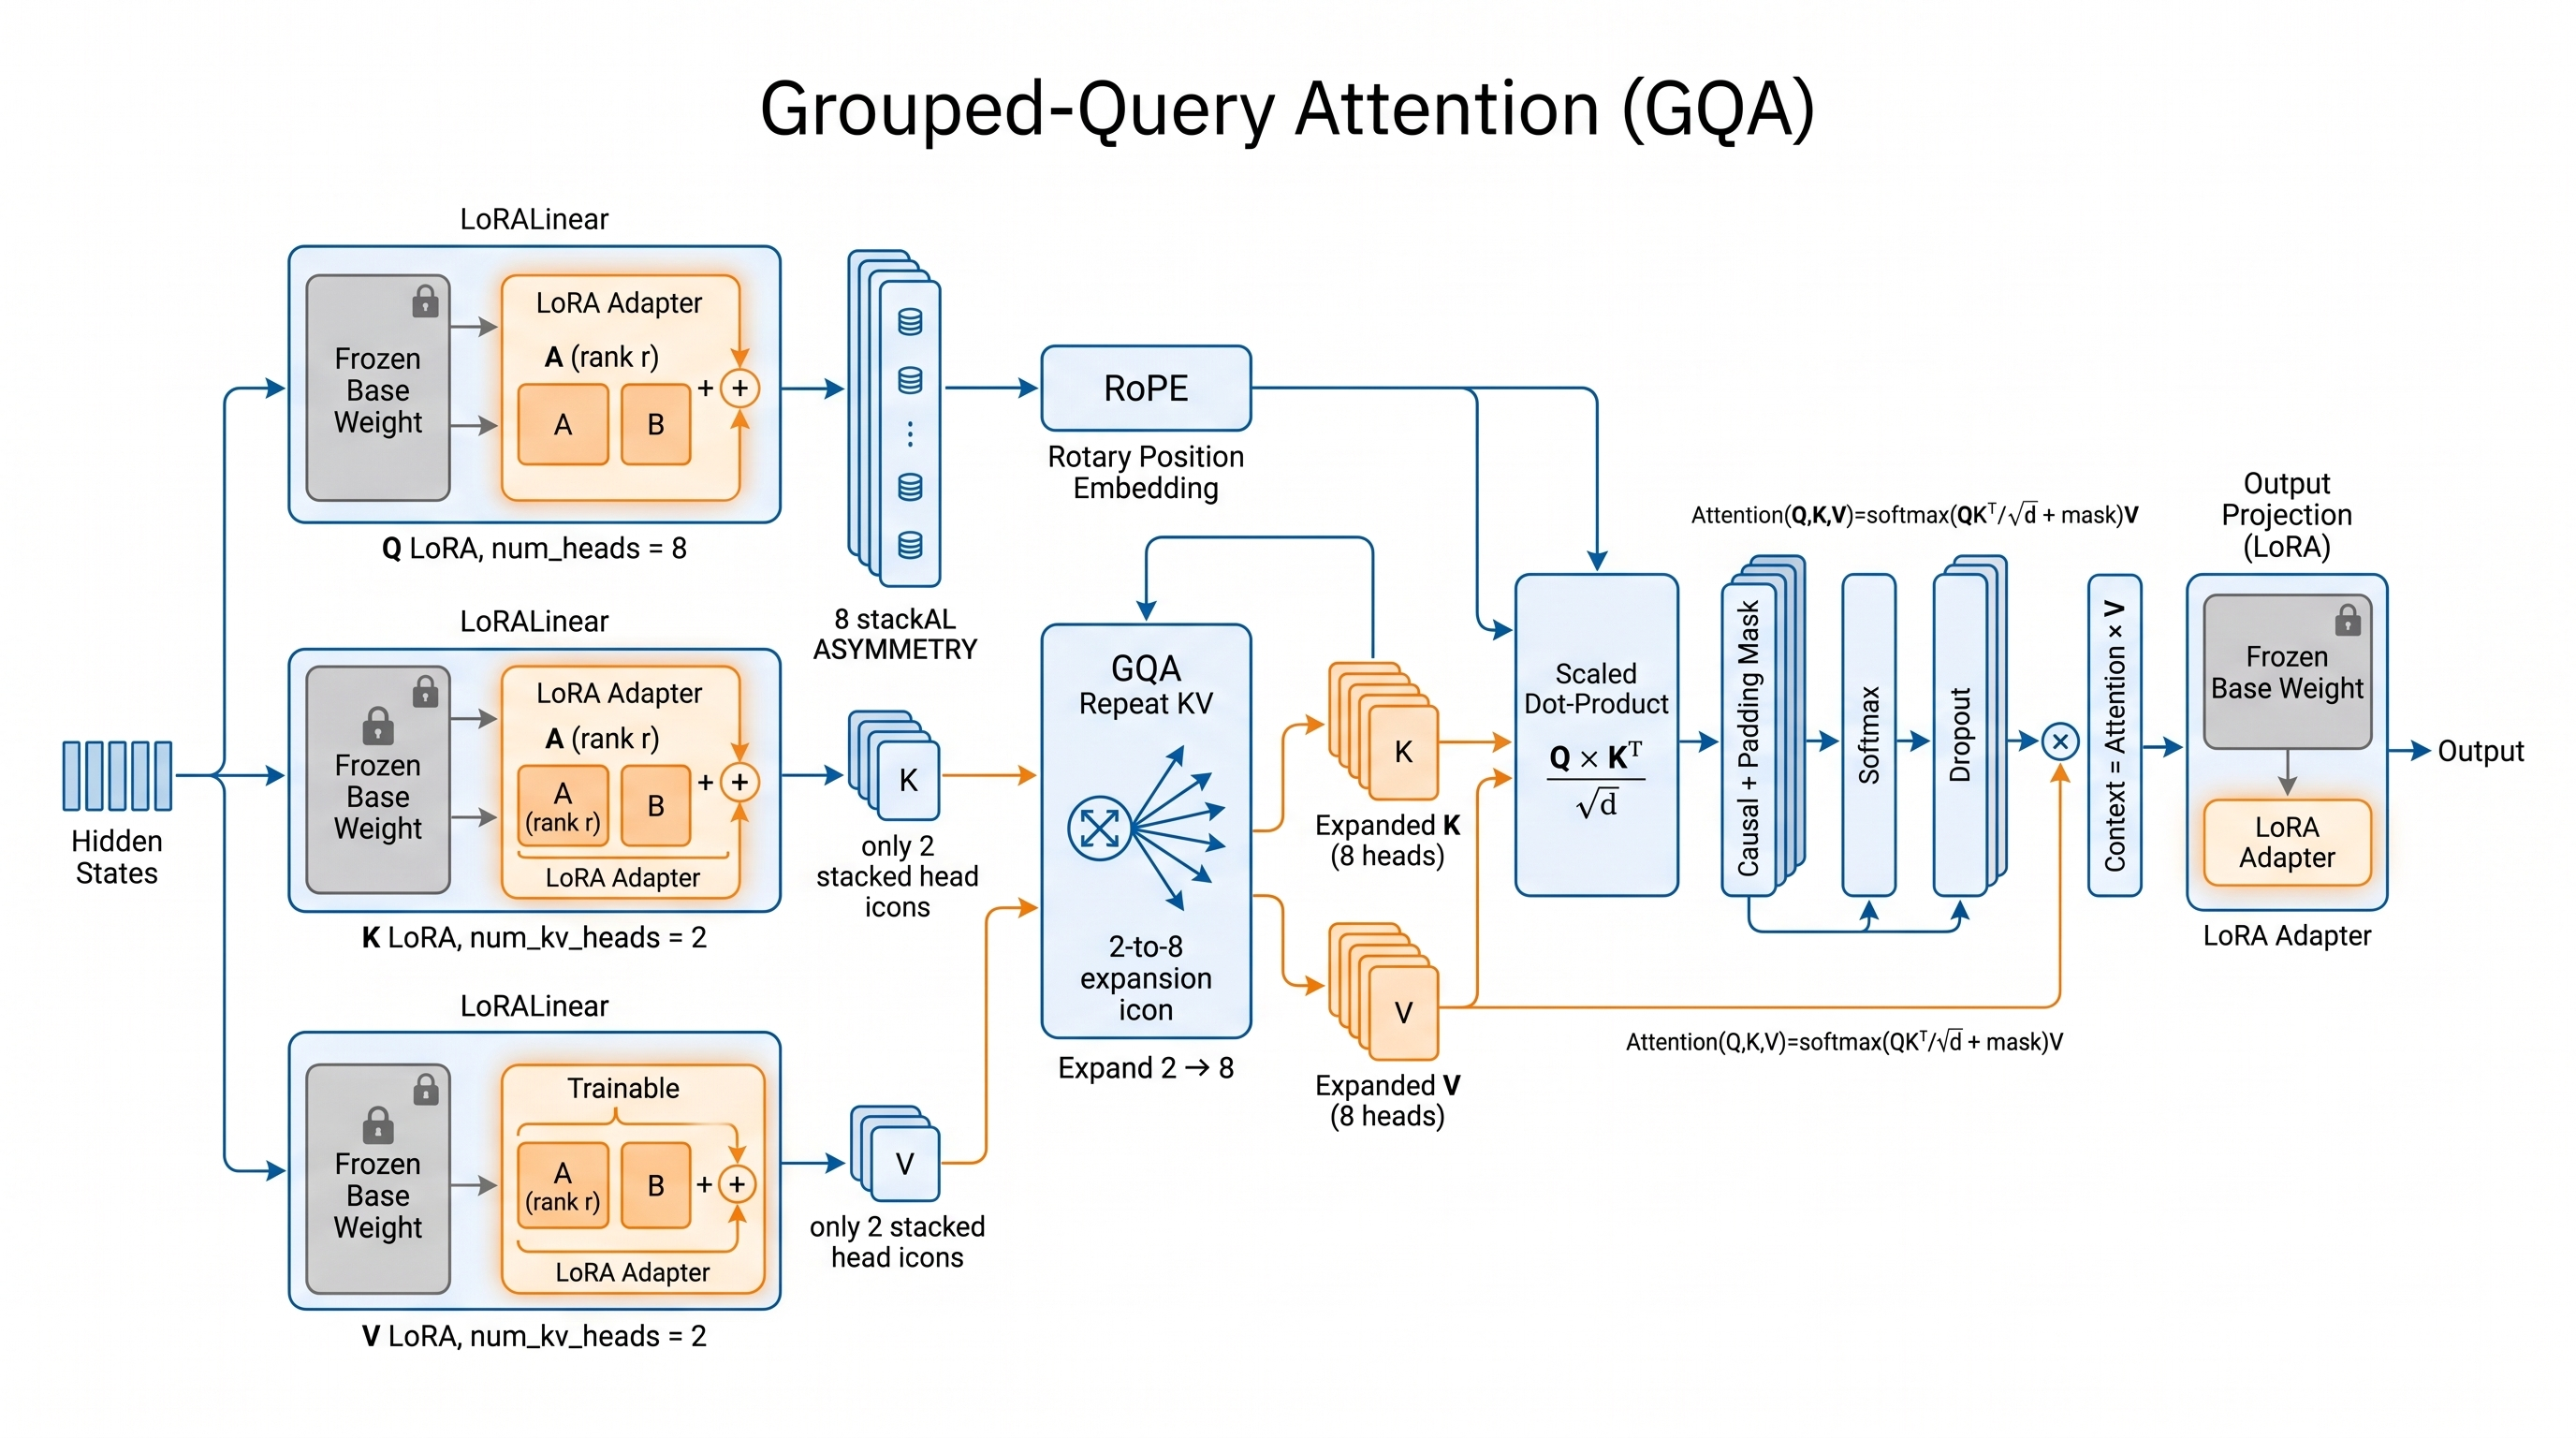
\includegraphics[width=0.92\textwidth]{img/arch_gqa_attention.jpeg}
\caption{دیاگرام ساختار معماری و جریان تانسوری ماژول \lr{(gqa\_attention)}}
\label{fig:arch_gqa_attention}
\end{figure}

\begin{figure}[H]
\centering
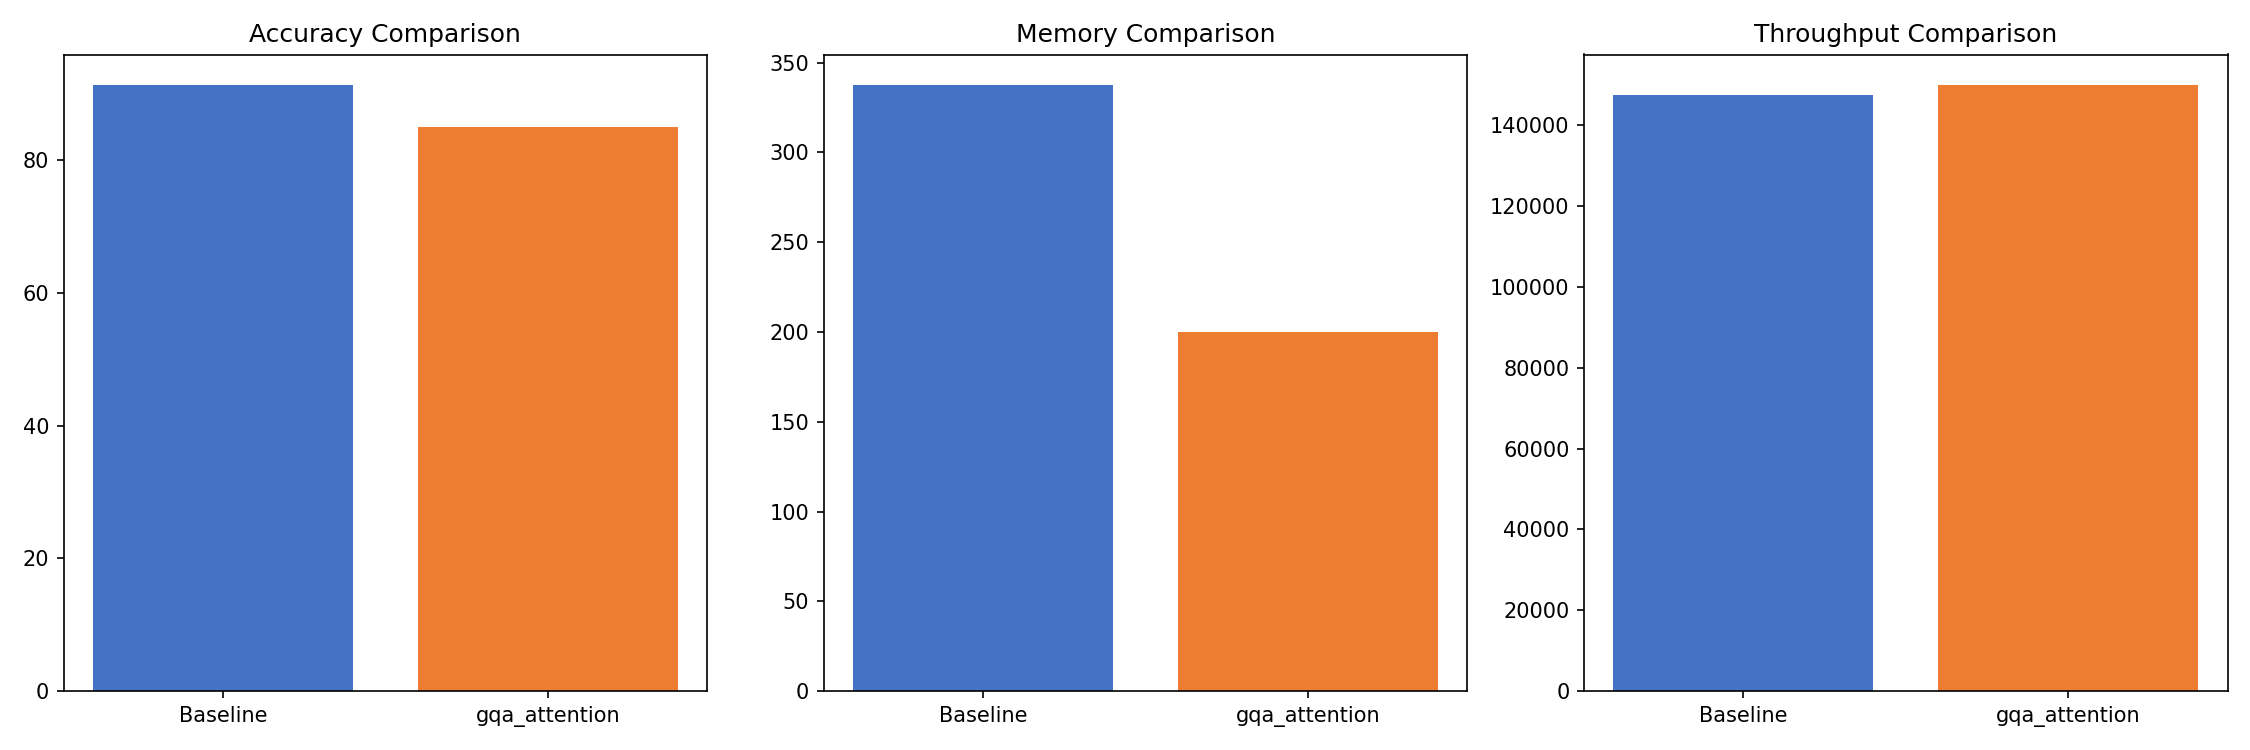
\includegraphics[width=0.92\textwidth]{img/comparison/gqa_attention_comparison.png}
\caption{نمودار ارزیابی مقایسه‌ای سه‌شاخصی مکانیزم در برابر خط مبنا \lr{(gqa\_attention)}}
\label{fig:comp_gqa_attention}
\end{figure}
